\documentclass[oneside, a4paper, onecolumn, 11pt]{article}

% Change this: Customize the title, author, advisor, abstract
\newcommand{\thesistitle}[0]{Advancements on Efficient Transformer Design}
\newcommand{\authorname}[0]{Francisco Moreira Machado Neto}

\newcommand{\supervisor}[0]{Dr. Van Minh Nguyen}
\newcommand{\supervisorinstitution}[0]{Huawei Technologies}

\newcommand{\abstracttext}[0]{%
The Transformer has been one of the major advancements in Machine Learning in recent years due to its flexibility and exceptional performance. 
With its wide adoption in particular its role in making the rise of large models such as ChatGPT, reducing its computational complexity has become an important matter of interest for recent research. In this thesis report, we first survey the foundational concepts of Transformers, highlighting its attention mechanism, to establish a comprehensive understanding of the architecture. We then delve into approaches focused on improving the efficiency of the Transformer: Binarization and Linear Attention Transformers. First, we establish a general framework for these innovations. Second, we highlight some notable adaptations of these techniques. Finally, we discuss benchmarks and possible future research directions.
}

\usepackage[
  left=2cm,top=2.0cm,bottom=2.0cm,right=2cm,
  headheight=17pt, % as per the warning by fancyhdr
  includehead,includefoot,
  heightrounded, % to avoid spurious underfull messages
]{geometry}


\usepackage[T1]{fontenc}
\usepackage{amstext}
\usepackage{amsmath}
\usepackage{amssymb}
\usepackage{url}
\usepackage{graphicx}
\usepackage{wrapfig}
\usepackage{caption}
\usepackage{subcaption}
\DeclareCaptionLabelFormat{nocaption}{}
\usepackage{enumerate}
\usepackage{paralist}
\usepackage{xspace}
\usepackage{color}
\usepackage{times}
\usepackage{tikz}
\usepackage{circuitikz}
\usepackage{bbm}
\usepackage[colorlinks,linkcolor=blue]{hyperref}
% \usepackage[colorinlistoftodos,prependcaption,textsize=normal]{todonotes}
\usepackage{pdfpages}
\usepackage{fancyhdr} %% For changing headers and footers

\usepackage{titling}
\usepackage[nottoc,numbib]{tocbibind}

%% \predate{}
%% \postdate{}
%% \date{}
%% \author{\authorname}
\newcommand{\softmax}{\text{Softmax}}
\DeclareMathOperator*{\argmin}{arg\,min}
\newcommand{\relu}{\text{ReLU}}
\def\app#1#2{%
  \mathrel{%
    \setbox0=\hbox{$#1\sim$}%
    \setbox2=\hbox{%
      \rlap{\hbox{$#1\propto$}}%
      \lower1.1\ht0\box0%
    }%
    \raise0.25\ht2\box2%
  }%
}
\def\approxprop{\mathpalette\app\relax}

\begin{document}

%\title{\thesistitle}

%\maketitle

% Max 10 lines.
%\noindent \paragraph*{Abstract}
%\abstract

\hspace{0pt}
\vfill

\begin{center}


\includegraphics[width=0.3\textwidth]{logo-EP-vertical}

\vspace*{2em}
%
{\large
\textbf{\'Ecole Polytechnique}

\vspace*{1em}
\textit{BACHELOR THESIS IN COMPUTER SCIENCE}


\vspace*{3em}
{\Huge \textbf{Advancements on Efficient \\ Transformer Design}}
\vspace*{3em}



\textit{Author:}

\vspace*{1em}
\authorname{}, \'Ecole Polytechnique

\vspace*{2em}
%
{\textit{Advisor:}}

\vspace*{1em}
\supervisor{}, \supervisorinstitution{}
}

\vspace*{2em}
\textit{Academic year 2023/2024}

\end{center}

\vfill
\hspace{0pt}

\newpage

\vfill
\noindent\textbf{Abstract}\\[1em]
%
\fbox{
\parbox{\textwidth}{
\abstracttext{}
}
}
\vfill


\newpage

% Setting up the header
\pagestyle{fancy}
%\renewcommand{\headrulewidth}{0pt} % Remove line at top
%\renewcommand{\headrulewidth}{0.4pt}% Default \headrulewidth is 0.4pt
\lhead{\authorname}
%\chead{\acronym}
\rhead{\thesistitle}



\newpage
\tableofcontents
\newpage

\section{Introduction}

Transformers \cite{vaswani2023attention} was introduced in 2017 and since then has powered many of the recent advancements in Artificial Intelligence (AI). Inspired by the attention mechanism for LSTMs \cite{10.1162/neco.1997.9.8.1735}\cite{bahdanau2016neural}\cite{luong2015effective}\cite{kim2017structured} that was ubiquitous for sequence-to-sequence (seq-to-seq) tasks,  Vaswani et al. proposed a model architecture that removed the recurrent network often associated with it, and relied entirely on attention for the sequence modeling. In doing so, the Transformers architecture deals with one of the fundamental bottlenecks of recurrent networks, the limited parallelization during training due to the sequential nature of dependencies. On the other hand, the Transformer can be efficiently parallelized which allows not only for faster training but also for deeper networks with more representational power.


Transformer-based models have been widely adopted in diverse fields,
such as natural language processing (NLP) and computer vision (CV), achieving state-of-the-art on various tasks. As such, there is a rich variety of research dedicated to applications and fundamental improvements to its original formulation. Alongside clever engineering, the strong scaling ability of Transformer-based models has played a big part in its success, with most of the models with billions of parameters being based on this architecture. Particularly, NLP-related tasks have been dominated by Transformer-based pretrained large language models (LLMs).

These increasingly larger models have demonstrated significant capabilities, however their sheer volume of parameters easily reaching hundreds of billions are associated with enormous computational and memory expenses. That means that without a significant redesign, these models have limited deployability for edge devices such as personal computers and mobile phones. Indeed, if we take the case of LLaMa2-70B model \cite{touvron2023llama}, it requires 150GB of storage in its default 16-bit floating point format, which is far beyond what any edge device realistically can afford to run. These surreal requirements are one of the reasons the search for more efficient Transformers-like models has been on the rise.

An efficient design results in less training time, and less costs for training and inference in the form of processing units and energy, while allowing for even more powerful models or enabling new applications. One example of this is telecommunications and wireless, in which performance is a major factor in the relevancy of a technology. Another one is for medical tasks, in which on-device inference would solve many of the privacy-related concerns of the technology. 

A multitude of techniques has been applied to obtain efficient Transformer models, such as model compression, sparsification of what is called the "attention matrix", or memory mechanisms to process sub-sequences separately. While many of these can be successfully applied to some scenarios, during this report we will focus on two promising approaches: Quantization and Linear Attention.

Quantization is a form of model compression that represents model weights and intermediate features of the model with fewer bits. For example, as we mentioned above, LLaMa2-70B is commonly used with weights in float16 format rather than full precision (float32), which reduces half the memory footprint of the model. Most quantization approaches focus on more aggressive compression, with $8, 4,$ or $1$ bit integers for weights and/or activations of the model. In that way not only the memory requirements are drastically reduced, but also more efficient operations are used with integer operands. In this report, we will focus on approaches pushing for binary quantization, i.e. $1-$bit representations, due to the promise of a $32$x reduction in storage and the elimination of expensive multiplication in favor of bit-wise operations. Notably, binary neural networks are claimed to provide energy consumption improvements of between $100-1000$x over full precision counterparts \cite{energy7929192}, further motivating the exploration of this approach.

The Linear Attention method for Transformers consists of a kernel-based formulation of the attention mechanism of Transformers. As we will develop in section \ref{sec:transformers}, the global scope of the attention mechanism results in a quadratic complexity in computations and memory consumption with relation to the sequence length, which is one of the main bottlenecks of the original formulation. To tackle this, linear attention uses feature maps and associativity of matrix products to calculate an alternative formulation of the module.

\section{Transformers}
\label{sec:transformers}
This section provides an overview of the Transformer model architecture as described by \cite{vaswani2023attention}, later referred to as Vanilla Transformer. This formulation is designed for seq-to-seq tasks and consists of an encoder and a decoder. The encoder maps an input sequence of embedded representation of words $(x_1, \ldots, x_L)$ to an intermediate representation $(z_1, \ldots, z_L)$. This intermediate representation is then fed to the decoder which then generates the output sequence $(y_1, \dots, y_M)$ one at a time in an auto-regressive manner. Informally, during the optimization process, the encoder learns embeddings of the input distribution, while the decoder learns to conditionally generate samples from the desired output distribution.

\begin{figure}[h]
\captionsetup[subfigure]{labelformat=nocaption}
\centering
\begin{subfigure}[b]{0.4\textwidth}
    \centering
    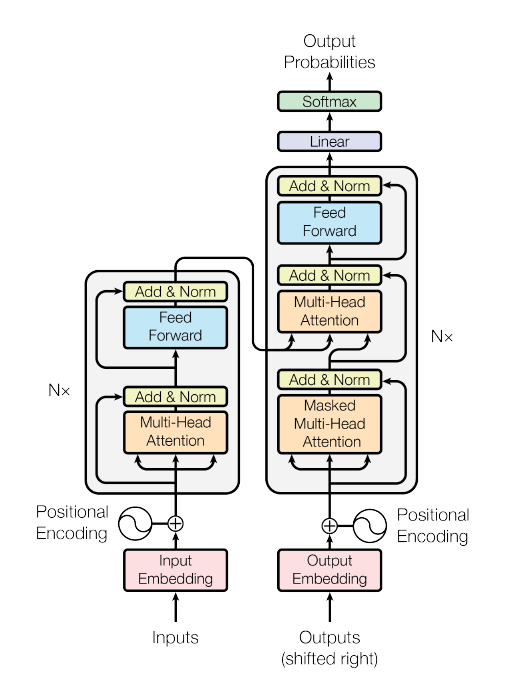
\includegraphics[width=\textwidth]{images/vanilla-arch.png}
    \caption{}
    \label{fig:vanilla-arch}
\end{subfigure}
\begin{subfigure}[b]{0.4\textwidth}
    \centering
    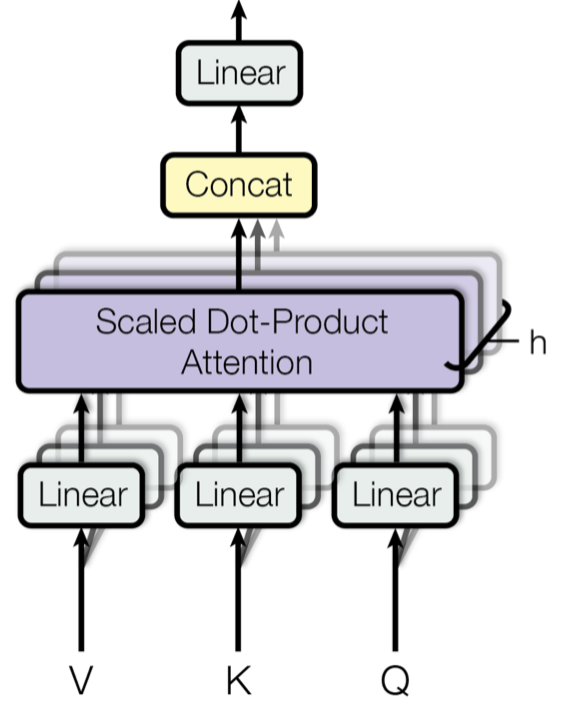
\includegraphics[width=0.9\textwidth]{images/multi-head.png}
    \caption{}
    \label{fig:multi-head}
\end{subfigure}
\caption{Transformers Architecture (a) and Multi-Head Attention (b) \cite{vaswani2023attention}}
\end{figure}

In order to describe the encoder and decoder of the Transformer architecture, we first need to understand the attention mechanisms and position-wise feed-forward layers.

\subsection{Multi-Head Attention}

Attention is the mechanism used by this architecture to capture dependencies between different positions within a sequence by attending to all positions simultaneously. Mathematically, this is represented by the function 
\begin{equation}
    A(Q, K, V) = \softmax\left(\frac{QK^\top}{\sqrt{d_k}}\right) V,
\end{equation}
where $Q \in \mathbb{R}^{m \times d_k}$ is the query matrix, $K \in \mathbb{R}^{n\times d_k}$ is the key matrix, and $V \in \mathbb{R}^{n \times d_k}$ is the value matrix. Conceptually, attention outputs the relevant values given a query to a set of key-value pairs by considering the similarity between the queries and the keys and then obtaining the values corresponding to the most similar keys. The product of $QK^T$ is scaled by $1/\sqrt{d_k}$ due to empirical observations that the unnormalized operation has values in regions of small gradients for the softmax function.

Additionally, to obtain the matrices $Q, K,$ and $V$, generally, an attention mechanism applies a linear map to the inputs $X_Q, X_K,$ and $X_V$, i.e. $Q = X_QW_Q, K=X_KW_K, V=X_VW_V$ for three learnable matrices $W_Q, W_K \in \mathbb{R}^{d \times d_k}, W_V \in \mathbb{R}^{d \times d_v} $. It is the convention to take $d_v = d_k$.


What we just described is called an \textit{Attention Head} and, as the name indicates, the multi-headed attention stacks several attention heads with unique sets of parameters in parallel. The outputs $A_1, \ldots, A_h$ of $h$ heads are then concatenated along the embedding dimension. It is the convention to set $h = d / d_k$ in order to keep the embedding dimension constant throughout the layers for easiness of stacking.

Multi-head attention has three main variants used for the encoder and decoder:
\begin{itemize}
    \item \textbf{Self-Attention:} This is the attention block used for the encoder. It sets $X_Q = X_K = X_V = X$, where $X \in \mathbb{R}^{L \times d}$ is the input of the encoder block.
    \item \textbf{Masked Self-Attention:} This is the first attention block used for the decoder. It also has $X_Q = X_K = X_V = X$ where $X \in \mathbb{R}^{M \times d}$ is the input of the decoder block, but in this variant, the positions are only allowed to attend to earlier positions in the output sequence. This is done by masking future positions to $-\infty$ before the softmax calculation.
    \item \textbf{Encoder-Decoder Attention:} This is the second attention block used for the decoder. It takes as input $X_Q$ the output of the masked self-attention (after residual connection and normalization as discussed later) and $X_K = X_V = Z$, the output of the encoder stack. This is meant to add the context of the input sequence to the decoder.
\end{itemize}


\subsection{Position-Wise Feed-Forward Network}

Attached to the output of the attention mechanisms, the Transformer architecture also includes a fully connected feed-forward network applied to each position of the input sequence separately but with the same weights. It consists of two linear layers connected by a ReLU activation. The inner-dimension is denoted by $d_{ff}$ and is generally taken as $d_{ff} = 4d$. It can still be represented by tensordot operations as:
$$
FFN(X) = ReLU(XW_1 + b_1)W_2 + b_2.
$$ 

Notice that while the attention mechanisms described above capture dependencies between positions, this block embeds positions independently.

\vspace{2em}

Now that we have introduced the two main components, we can describe the full architecture. As represented in figure \ref{fig:vanilla-arch}, both the encoder and decoder are composed of $N$ layers of identical blocks stacked. They have \textit{Add \& Norm} sub-blocks, which represent a residual connector with the input of the preceding block, followed by layer normalization \cite{ba2016layer}. After each multi-head attention of the position-wise feed-forward layer, an Add \& Norm layer is attached.
\begin{itemize}
    \item \textbf{Encoder Block:} Consists of a multi-head self-attention mechanism and a position-wise feed-forward layer.
    \item \textbf{Decoder Block:} Consists of a multi-head masked self-attention mechanism, a multi-head encoder-decoder attention mechanism as described above, and a position-wise feed-forward layer.
\end{itemize}

Although it remains to describe a few components, the key components that will be further explored during this report are highlighted until now: Attention, Encoders, and Decoders.

As for the remaining components, we first have the tokenization. It consists of the process of turning input text into raw atomic data. These raw data
correspond to the basic elements from which the model estimates meaningful interactions.
This is done by assigning an identifier to a word, a character within words or segment
of words (subwords). Starting from a large corpus of text, the tokenizer extracts the
subwords, or tokens, to use for id assignation. As a result, it retrieves a map that relates
tokens with ids. Afterwards, this map is used to tokenize sentences that serve as inputs
to the model.

Once all data is tokenized, we have embeddings for inputs and outputs (inputs for decoder) that transform the tokens to vectors of dimension $d$ with linear transformations. This embedding is added to a positional encoding to inject information about position of tokens. These are then ready to be fed to the model.

Finally, to obtain a probability distribution for the predicted next token of the sequence, the output of the last decoder layer is passed through a linear layer with softmax activation.

\subsection{Model Adaptation}

Generally, the usage of the Transformers architecture we just described can be divided into three different categories:
\begin{itemize}
    \item \textbf{Encoder-Decoder:} The full Transformer architecture. This is typically used for seq-to-seq tasks such as machine translation. 
    \item \textbf{Encoder-only:} Only the encoder part of the Transformer architecture is used, and the encoder output is generally used to embed the input sequence. This is generally used for classification tasks. Notably, the BERT \cite{devlin2019bert} family of models is an example of this.
    \item \textbf{Decoder-only:} Only an adapted decoder is used, with the removal of the Encoder-Decoder attention mechanism. This is commonly used for generative tasks. Notably, the GPT \cite{brown2020language} family of models used a decoder-only architecture.
\end{itemize}

Beyond architectural changes, a great variety of Transformer-based models introduce diverse modifications to the model pipeline. Remarkably, since the Transformer is a flexible architecture and makes few implicit prior assumptions on the input data distribution, it is generally hard to train a model on small-scale data. This issue has been widely tackled by self-supervised pre-training on large datasets \cite{devlin2019bert}\cite{brown2020language}, which allows large networks to be trained without the need to acquire expensive manually labeled data, e.g. in the case of NLP tasks. 

Two classes of pre-training tasks that have been successfully used are \textit{Fill the Blanks} and \textit{Contrastive Learning}. For the former, the task is to predict a hidden or masked part of the input sequence or reverse a permutation applied to the input, which aims to teach the model bidirectional context leveraging. The latter consists of presenting the model with three inputs, two of which are "compatible" and one other that is not; the task is then for the model to detect which two of the three are compatible. This is generally implemented by applying a transformation to the data that is desirable for the model to be invariant. An example of it is \textit{Next Sentence Prediction} which is used for BERT, which helps capture sequence-to-sequence relationships. 

In the era of Large Language Models (LLMs), pre-trained models became the standard. A single general-purpose pre-trained model on large-scale data can be leveraged by fine-tuning the model for a wide-variety of downstream tasks, which has been powering many of the industry applications of NLP.

\subsection{Computational Costs}
Now, let us analyze the computational costs of transformers. We will restrict the study to a single encoder block, for the sake of simplicity, however it easily extends to the decoder block and a stack of blocks of either. Let us use the same notation as before, with an input sequence of length $L$, embedded space of dimension $d$, $h$ attention heads, embedding space for the keys $d_k$ ($d_k h = d$), and let $M$ be the length of the output embedding. The layer normalization and residual connection have linear complexity for each head, thus both memory and computational complexity is $O(h d_k L + Ld) = O(Ld)$.

\begin{table}[ht!]
\centering
\begin{tabular}{l c c} 
 \hline
    Module & Computation & Memory \\ [0.5ex] 
 \hline
 (Masked) Self-Attention & $O(L^2d)$ & $O(Ld + hL^2)$ \\ 
 
 Encoder-Decoder Attention & $O(LMd)$ & $O(Md + hLM)$ \\
 
 FFN & $O(Ld^2)$ & $O(Ld)$ \\

 \hline
\end{tabular}
\caption{Complexity of Attentions and Position-Wise Feed-Forward}
\label{table:1}
\end{table}

Moreover, both the self-attention and position-wise feed-forward have complexities dominated by matrix multiplications. For the former, the multiplication of $\softmax(QK^\top / \sqrt{d_k})$ of shape $L \times L$  with $V$ of shape $L \times d_k$ takes $O(L^2d_k)$ operations and $O(Ld_k)$ to store the result, while computing $QK^\top$ also takes $O(L^2d_k)$ operations and requires $L^2$ of memory to store the result. Repeating this over the $h$ heads gives the complexities as described in table \ref{table:1}. Note that this simply extends to masked self-attention as the operations are essentially the same, and similarly to encoder-decoder attention.

For the position-wise feed-forward layers, assuming the convention that $d_{ff} = 4d$, the tensor-dot described before only requires $O(Ldd_{ff}) = O(Ld^2)$ operations, with $O(Ld)$ memory is sufficient to store the partial results.



\vspace{0.5em}

Now that we analyzed the costs of a single pass through a transformer layer, let us recall that during \textit{inference} we generate one token at a time. This adds a degree to the final computational order of magnitude resulting in $O(LM^2d + M^3d)$ complexity as the decoder has two types of attention. This issue can however be mitigated through clever re-utilization of computations of the previous steps, as formulated in   appendix \ref{sec:appendix}.

\vspace{0.5em}

It is important to remark that this represents the total number of computations per layer, however, these can be efficiently parallelized due to basically no sequential dependency of computations within each module. This is in stark contrast with recurrent networks, which can be argued to have better total complexity but have a higher number of sequential operations.

Moreover, although Transformers improve training speed drastically through improved parallelism, the Self-Attention module has an alarming quadratic complexity in relation to the length of the sequence in both computation and memory. 
This is prohibitive for handling large corpus of text such as codebases, articles, or books, and generally limits the scalability of the architecture. 
Although the overall architecture also has a quadratic number of computations with relation to the embedding dimension $d$, this is a constant set as a hyperparameter, while the input sequence length can be variable and for modern applications it usually holds that $L_{max} \gg d$. With this in mind, a wide variety of novel approaches have been proposed in recent years for efficient architectural modifications. Notably, we will explore two techniques for such: Linear Transformers and Quantization.

\newcommand{\sign}{\text{sign}}
\newcommand{\bool}{\text{bool}}
\section{Binarization}

Quantization has received attention as one of the most promising techniques to reduce the model size of LLMs. Not only does this technique have very promising benefits, but also it has been greatly successful in some applications \cite{liu2020reactnet}\cite{rastegari2016xnornet}. Although the idea of reducing the bit-width of weights and/or activations is relatively simple, successfully implementing it is not as much. We are particularly interested in extreme quantization, i.e. binarization, as it not only promises a 32x times improvement in memory footprint but also enables the substitution of expensive floating point arithmetic with highly efficient binary operations. However, with its higher memory reduction and arithmetic cost benefits comes also a series of problems in representative capabilities and difficulty of optimization. In this section, we will establish the fundamentals of model binarization and highlight a few clever methods that were applied to Transformer-based LLMs.

\begin{figure}[!ht]
\centering
\resizebox{0.8\textwidth}{!}{%
\begin{circuitikz}
\tikzstyle{every node}=[font=\normalsize]
\draw  (2.5,17) circle (1.25cm);
\node [font=\Large] at (5.5,17.3) {Pre-Train};
\draw  (8.75,17) circle (1.25cm);
\draw  (15,19.5) circle (1.25cm);
\draw  (15,14.5) circle (1.25cm);
\draw  (21.25,14.5) circle (1.25cm);
\draw [short] (10,17) -- (11.25,19.5);
\draw [short] (10,17) -- (11.25,14.5);
\draw [->, >=Stealth] (11.25,19.5) -- (13.75,19.5);
\draw [->, >=Stealth] (11.25,14.5) -- (13.75,14.5);
\draw [->, >=Stealth] (16.25,14.5) -- (20,14.5);
\draw [->, >=Stealth] (3.75,17) -- (7.5,17);
\node [font=\Large] at (12.5,19.85) {Fine-Tune};
\node [font=\Large] at (12.5,14.85) {Fine-Tune};
\node [font=\Large] at (12.4,19.1) {QAT};
\node [font=\Large] at (18,14.85) {PQT};
\node [font=\LARGE] at (2.5,17) {$M_0^{FP}$};
\node [font=\LARGE] at (8.7,17) {$M_1^{FP}$};
\node [font=\LARGE] at (15,19.5) {$M_2^{B}$};
\node [font=\LARGE] at (15,14.5) {$M_3^{FP}$};
\node [font=\LARGE] at (21.3,14.5) {$M_4^{B}$};
\end{circuitikz}
}%
\caption{Scheme of training procedure for QAT and PTQ. The FP superscript means the model is trained in full precision, while B means it is binarized.}
\label{fig:quant_scheme}
\end{figure}

\newpage
There are two main classes of quantization methods: 
\begin{itemize}
    \item \textbf{Post-Training Quantization (PTQ): } Consists of taking an already trained model and quantizing its weights as well as establishing a strategy for reducing the bit-width of input and activations on inference. These are generally more practical to use since they require less computational power and overall changes to the training pipeline.

    \item \textbf{Quantization-Aware Training (QAT): } Consists of designing a new pipeline for training the model with quantization in mind. These have the potential for better performance, but come with the cost of additional training the models, making it a much more costly approach.    
\end{itemize}

Notably, when applying quantization to language models, both methods start from a pre-trained model, as indicated in figure \ref{fig:quant_scheme} by $M_1^{FP}$, to avoid the massive cost associated with training from these networks from scratch. The methods then differ starting from the fine-tuning process. In QAT, we fine-tune the model taking into consideration the quantization procedure. In PQT, we first fine-tune the model (or take a fully trained one) and then apply a quantization strategy for its weights and activations.

\subsection{General Framework}
% Up to my knowledge at the time of writing, the most relevant binary PTQ focuses on the BERT \cite{devlin2019bert} architecture, which is an encoder-only Transformer-based model, however, the techniques established can be leveraged with minor modifications to other types of Transformer.

We will start by establishing a baseline approach, inspired by \cite{Qin2022bibert}, as it describes many common techniques for binary PTQ and QAT. Key to the formulation of binary networks is the $\sign(x)$ function, defined as
\begin{equation}
    \sign(x) = \begin{cases}
        1, & \text{if } x \geq 0 \\
        -1, & \text{otherwise}
    \end{cases},
\end{equation}
for the forward pass, and the Straight-Through Estimator (STE)\cite{bengio2013estimating} for the backward pass. Indeed, as the name suggests, STE allows the full gradient to pass during the backpropagation with the identity function used to propagate the gradient. Notice that this function will be frequently used to bring activations and weights to $\{-1, 1\}$, the standard pair of numbers used for binarization.

Moreover, we must establish how to binarize the pre-trained weights. As all weights of transformers come from linear fully connected layers, we can focus on this type of parameter. Given a full-precision weight matrix $W$, we would wish to find $W_B$ with values in $\{-1, 1\}$ and a scaling factor $\alpha \in \mathbb{R}^+$ to minimize the approximation error $\|XW - \alpha XW_B \|$ over all possible inputs $X$. The introduction of $\alpha$ as a full-precision scaling factor has the purpose of reducing drastically the quantization errors \cite{rastegari2016xnornet} while preserving the benefits of binary storage and efficient matrix multiplications with xnor and bitcount operations.

This motivates us to solve the following optimization problem, as done by \cite{rastegari2016xnornet} 

\begin{equation}
\label{eq:optim_bin}
    \min_{\alpha, W_B} \| W - \alpha W_B \|^2.
\end{equation}

We may assume for simplicity that both $W$ and $W_B$ are vectors on $\{-1, 1\}^k$ for some $k$ by flattening them out, as it does not change the optimization problem. With this, we can expand to get
\begin{align}
    \min_{\alpha, W_B} W^\top W - 2\alpha W^\top W_B + \alpha^2 W_B^\top W_B,
\end{align}
which in turn we can reduce as $W_B^\top W_B = n$ and $W^\top W$ is a fixed constant, so the problem becomes
\begin{equation}
    \max_{\alpha, W_B} 2\alpha W^\top W_B - \alpha^2 n,
\end{equation}
in which the optimal solution for $W_B$ can achieved independently of $\alpha$ (as it is positive) by 
\begin{equation}
    W_B^* = \max_{W_B} W^\top W_B = \sign(W).
\end{equation}

Finally, we obtain $\alpha^*$ as 
\begin{equation}
    \alpha = \cfrac{W^\top W_B^*}{n} = \cfrac{W^\top \sign(W)}{n} = \cfrac{\sum_{i=1}^n |W_i|}{n},
\end{equation}
so we have a fixed formula to compute the optimal binary approximation with a scaling factor given the pre-trained weights. 

Moreover, before introducing what is called the bi-linear layer, we discuss yet another standard optimization when doing quantization. It is common practice to normalize the weights to zero-mean before applying the quantization function, for retaining representation information \cite{qin2020forward}. We therefore use the same identities as before for $\alpha$ and modify $W_B$ by taking $W' = W - \mu(W)$, with $\mu$ being the mean function.

Now we are ready to define a binary alternative to a pre-trained linear layer as:
\begin{equation}
    \text{bi-linear}(X) = \frac{1}{n}\|W\|_{\ell_1} (\sign(X) \otimes \sign(W')).
\end{equation}

Notice that here we binarize $X$ by just the sign activation for a baseline approach (indeed, one can prove that by assuming the data has a centered Gaussian distribution, the sign function maximizes the entropy). Moreover, we denote the matrix multiplication by $\otimes$ as this is an operation that can be fully computed through efficient binary operations.

\vspace{1em}

Now to define a fully binary transformer block, it suffices to substitute the linear embedding to obtain $Q, K,$ and $V$ for the bi-linear layer, as well as the position-wise feed-forward network. We then obtain 
\begin{equation}
   Q_B = \sign(Q), Q_K = \sign(K), A = \frac{1}{\sqrt{d_k}}\left( Q_B \otimes K_B^\top \right), 
\end{equation}
and ultimately the result of self-attention can be obtained by concatenating $\sign(\softmax(A))$. Notice however that as softmax is a positive function, this last term will result in all entries being $1$, thus we introduce learnable shift parameters $\tau_i$ and rewrite the output of multi-head attention as:
\begin{equation}
    \text{MHA}(X) = \text{Concat}(\sign(\softmax(A_1) - \tau_1), \ldots, \sign(\softmax(A_h) - \tau_h)).
\end{equation}


\vspace{1em}

The final key approach to quantization is \textit{knowledge distillation} (KD)\cite{hinton2015distilling}. The technique consists of training a student network to mimic the behavior of a teacher network, usually to compress or transfer knowledge to more efficient networks. This is achieved by adding an extra term to the loss function that incentivizes mimicking a certain behavior of the teacher network. Two main classes of KD methods can be applied to quantization:

\begin{itemize}
    \item \textbf{Logit-based KD:} This method adds an objective for the student model to match the output probability distribution of the teacher one. To illustrate the objective of this method, we denote the logits output of the teacher and student network as $z^s, z^t$, i.e., the outputs before applying a softmax layer. Now let $p^s = \softmax(z^s), p^t = \softmax(z^t)$, then our objective function is the KL divergence between the teacher and student probability distribution as
    \begin{equation}
        \mathcal{L}_{logits} = KL ( p^t || p^s).
    \end{equation}

    \item \textbf{Hint-based KD:} This method attributes as an objective to match an intermediate feature of the teacher network. This can be formulated by considering a corresponding intermediate feature $F^s, F^t$ of the student and teacher networks, respectively, and considering a certain distance measure $\mathcal{D}$, which is taken as the mean squared error (MSE) unless specified otherwise, and finally
    \begin{equation}
        \mathcal{L}_{hint} = \mathcal{D}(F^s, F^t).
    \end{equation}
\end{itemize}

Different approaches to binarization combine these two modes of distillation differently. KD is considered to be an essential enhancement to alleviate the representational limitations and performance drop of extreme bit-width settings. 

For a baseline, we consider a distillation that takes the cross entropy of the output of the teacher and student logits $z^t, z^s$, respectively, which we refer to as $\mathcal{L}_{cross}$, as well as three hint-based KD with intermediate features being, for the $i-th$ layer, the matrix $A$, the output of the MHA, and the hidden representations $Y$ which are of the Transformer block. These are represented as $\mathcal{L}^i_{A}, \mathcal{L}^i_{\text{MHA}}, $ and $ \mathcal{L}^i_{Y},$ respectively.
If we pick a design of $N$ layers of Transformer blocks, the total loss can be described as
\begin{equation}
    \mathcal{L}_{distil} := \mathcal{L}_{cross} + \sum_{i=1}^N \mathcal{L}^i_{A} + \mathcal{L}^i_{\text{MHA}} + \mathcal{L}^i_{Y}.
\end{equation}

\subsection{Related Progress}

With a general framework established, we can describe the key improvements made to it. We will first explore two QAT approaches to BERT as a base model:  BiBERT \cite{Qin2022bibert} and BiT \cite{liu2022bit}.

BiBERT suggests Bi-Attention as a replacement for the binarization for the attention mechanisms. The design choices are based on maximizing the information entropy of the binarized representations. The authors establish the statistical hardness of determining a parameter $\tau$ to maximize the information entropy $\mathcal{H}(\sign(\softmax(A) - \tau))$, which is q key parameter for the model's performance. Under assumptions of independence of the rows of $A$, they conclude that is approximately optimal to remove the softmax of the attention head and compensate for this removal by using $\bool(A)$ as the activation, where $\bool(x)$ is defined analogously to $\sign$ by attributing $1$ if $x \geq 0$ and $0$ otherwise. The Bi-attention can then be formulated as
\begin{equation}
    \text{Bi-Attention}(Q_B, K_B, V_B) = \bool \left( \frac{1}{\sqrt{d_k}} (Q_B K_B^\top )\right) V_B.
\end{equation}

BiBERT also includes a mechanism to tackle the optimization problems that arise from baseline distillation and binarization. The phenomenon of direction mismatch is a common problem for quantization problems, which consists of the optimization process resulting in undesired behavior by being insufficient for convergence or even harmful. This can be caused by the low precision of the parameters preventing the desired optimization directions. Upon studying how this mismatch relates to the bit-width on a theoretical scenario of Gaussian distributed inputs, the authors design a Direction Matching Distillation (DMD) scheme to remediate the mismatch.

The most severe direction mismatch occurs when computing the approximation error of $Q_BK_B^\top$ with relation to $Q K^\top$ (which is included in the $\mathcal{L}_A$), which is believed to be caused by the multiplication of two binarized activations. To remediate, the authors propose to distill directly the $Q$, $K$, and $V$, with the latter being motivated by a similar argument with relation to $\mathcal{L}_\text{MHA}$. To enable the comparison between $Q, K$, and $V$ and the binary counterparts, one first constructs similarity matrices given by 
\begin{equation}
    F_Q = \frac{QQ^\top}{\|QQ^\top\|},
    F_K = \frac{KK^\top}{\|KK^\top\|},
    F_V = \frac{VV^\top}{\|VV^\top\|},
\end{equation}
and similarly defined binary counterparts named $F_Q^B, F_K^B,$ and $F_V^B$. We finally introduce $\mathcal{L}_Q = \|F_Q - F_Q^B\|$ and analogously for the others to obtain
\begin{equation}
    \mathcal{L}_{distil} = \mathcal{L}_{cross} + \sum_{i=1}^N \mathcal{L}_Q^i + \mathcal{L}_K^i + \mathcal{L}_V^i + \mathcal{L}^i_Y.
\end{equation}

\vspace{1em}

BiT, on the other hand, makes the framework more flexible by allowing some intermediate features to have values in $\{0, 1\}^k$ rather than $\{-1, 1\}^k$. The authors confirm through ablation studies that when the full-precision network goes through positive activation functions, such as ReLU or Softmax, the binary counterpart obtains better performance when the binarization space is $\{0, 1\}^k$. Otherwise, if the hidden representation takes values in $\mathbb{R}^k$, the binarization space remains $\{-1, 1\}^k$ with the $\sign$ function. Indeed, if we assume such a space we can solve a similar optimization problem to eq. (\ref{eq:optim_bin}) and obtain
\begin{equation}
    X_B^* = \lfloor \text{Clip}(X - \mu(X), 0, 1) \rceil, \;\;\; \alpha^* = \frac{\| W \cdot \mathbbm{1}_{\{W \geq 0.5\}} \|_{\ell_1}}{|\{X \geq 0.5\}|},
\end{equation}
where $\text{Clip}(x, a, b) = \max(a, \min(b, x))$, $\lfloor \cdot \rceil$ is the nearest integer approximation, $\mathbbm{1}_{\{X \geq 0.5\}}$ is a vector containing $1$ if the equivalent entries of $X$ are greater than or equal to $0.5$ and $0$ otherwise, and $|\cdot|$ is the set cardinality function.

Moreover, they modify this binarization approach to be even more flexible by introducing a learnable threshold $\beta$ to the $\sign$ and $\text{Clip}$ activations. These are formulated as
\begin{equation}
    X_B^+ = \lfloor \text{Clip}( \frac{X^+ - \beta}{\alpha}, 0, 1) \rceil, \;\;\; X_B = \sign(X - \beta),
\end{equation}
in which we denote with the $+$ superscript the positive hidden representations. This approach also makes the $\alpha$ a learnable parameter which is initialized as $\alpha^*$.

Additionally, BiT includes two key modifications to the distillation process. First, the distillation objective is simplified to $\mathcal{L}_{distil} = \mathcal{L}_{cross} + \sum_{i=1}^N \mathcal{L}^i_{Y}$. Second, the distillation follows a multi-step approach, in which we gradually reduce the quantization level to finally obtain a binarized model, which aims to mitigate issues due to the drastic difference between high-precision teacher and low-precision models. Formally, the multi-step distillation follows a schedule $Q = \{ (b^1_w, b_a^1), \ldots (b^l_w, b^l_a) \}$ where $(b^i_w, b^i_a)$ represents that at the $i$-th step, we have a model with weights in bit-width $b^i_w$ and activations in bit-width $b^i_a$. By default, the schedule is taken as $Q = \{(32, 32), (1, 2), (1, 1)\}$.

\vspace{1em}

Now that we defined how the forward and backward pass work for BiBERT and BiT, it remains to discuss how the parameter update is made. For both methods, as well as many QAT variants, during the fine-tuning stage, the full precision parameters are still the ones being stored. The updates are then made to these with conventional optimizers, with the binary representation being obtained via the methods we established before. At the end of this process, only the binary representations are stored for the fine-tuned model. ,


\vspace{1em}

Now we explore one very recent binary PTQ method for LLMs: BiLLM \cite{huang2024billm}. In this constrained setting, the authors opt to binarize only the weights of LLMs, keeping the activations in their original precision, which is generally 16 bits.
With no usage of fine-tuning, the authors need to obtain a better understanding of the statistical properties of the weights and extract suitable properties from them. 
This is exactly what the authors use as a reference for this novel approach. Upon studying the distribution and Hessian matrix of weights, the authors make two key observations: 

\begin{enumerate}
    \item The Hessian matrix has a long-tail distribution. This is interpreted as a minor part of the weights having major significance for the LLM.
    \item The magnitude of the weights has a Gaussian-like distribution. This poses a major problem, as binarization results in severe quantization errors for such distributions \cite{jacob2017quantization}.
\end{enumerate}
   
To take into account point 1. which we just discussed, the authors propose to double the bit-width of what they call "salient" weights, which conceptually are those that are the most relevant to the network. Like that, these would be better approximated in the binarized network. For each layer, we deal with weights separately as follows, we first define the salience of each weight as (assume flattened weights for this definition)
\begin{equation}
s_i = \cfrac{w_i^2}{\mathbf{[H^{-1}]}^2_{ii}}.
\end{equation}

Now let us call $S$ the salience matrix, with the same dimensions as $W$, the weight matrix (by folding). For a structured choice of salient weights, we pick full columns to be the salient ones. From now on, let us assume that the columns of $W$ are ordered based on the sum of the columns of $S$. By denoting $W_{sal}, W_{uns}$ to be the weights of salient and non-salient columns, respectively, we can rewrite eq. (\ref{eq:optim_bin}) as
\begin{equation}
\label{eq:salient_optim}
    \min_{W_{sal}^B, W_{uns}^B, \alpha_{sal}, \alpha_{uns}} \|W - \text{Concat}(\alpha_{sal} W_{sal}^B, \alpha_{uns}W_{uns}^B) \|^2,
\end{equation}
with the $B$ superscript meaning the binary approximation, as usual. We can solve this in the same way as we did for eq. (\ref{eq:optim_bin}) by solving for the two sets of columns separately. Now it just remains to choose how many columns are salient. This is done by solving eq. (\ref{eq:salient_optim}) with the number of columns starting from $1$ and up to $k$, which is a hyperparameter, and picking the one with the lowest approximation error.

Upon selecting the salient columns, the authors opt to approximate them with double the bit-width but still with the binarization approach in mind. Indeed, instead of solving equation $(\ref{eq:optim_bin})$ for the salient columns, the residual approximation optimization optimizes in the following way
\begin{equation}
    \alpha_o^*, W_o^* = \argmin_{\alpha_o, W_0} \|W_{sal}^{FP} - \alpha_o W_o\|^2, \;\;\;  \alpha_r^*, W_r^* = \argmin_{\alpha_r, W_r} \|(W_{sal}^{FP} - \alpha_o W_o) - \alpha_r W_r\|^2.
\end{equation}

This results in the approximation for the full precision salient columns of $W$ as $W_{sal}^{FP} \approx \alpha_o W_o + \alpha_r W_r$. 

\vspace{0.5em}

For observation 2. as indicated above, the authors propose once again to split the non-salient weights into two sets that will be binarized separately, however this time both with bit-width 1. By identifying the Gaussian-like distribution of weights, we hope to divide the non-salient weights into two groups depending on their values. We define $I_c = [-p, p]$ to be the interval defining the group of \textit{concentrated} weights, and $I_c = I_s^{C}$ (the complementary interval) to define the group of \textit{sparse} weights. 

With this division, we can rewrite the optimization problem to find (again by assuming proper reordering)
\begin{equation}
   \alpha_c^*, \alpha_s^*, W_c^*, W_s^* =   \argmin_{ \alpha_c, \alpha_s, W_c, W_s} \| W_{uns}^{FP}- \text{Concat}(\alpha_cW_c, \alpha_sW_s) \|,
\end{equation}
which we know how to solve as discussed before. Therefore it only remains to choose an optimal $p^*$ to minimize the quantization error. The proposed process to find $p^*$ is by conducting a grid search on $[0, 9]$. 

\subsection{Benchmarks and Discussion}

As both BiBERT and BiT adapt the BERT base architecture, we can make a straightforward comparison of them. Moreover, BERT is well-suited for classification tasks, so generally, it is tested through classification tasks. We include here the classification accuracy performance on the GLUE \cite{wang2019glue} benchmark tasks, considering the results of the fully binarized BiT.

\begin{table}[ht!]
\small
\centering
\begin{tabular}{l c c c c c c c c c c} 
\hline
  Method & Size (Mb) & MNLI m/mm & QQP & QNLI & SST-2 & CoLA & STS-B & MPRC & RTE & Avg. \\
\hline
    BERT base & 418 & 84.9/84.5 & 91.4 & 92.1 & 93.2 & 59.7 & 90.1 &  86.3 & 72.2 & 83.9\\
    BiBERT & 13.4 &  66.1/67.5 & 84.8 & 76.0 & 90.9 & 37.8 & 56.7 & 78.8 & 61.0 & 68.8 \\
    BiT & 13.4 & 79.5/79.4 & 85.4 & 86.5 & 92.3 & 38.2 & 84.2 & 88.0 & 69.7 & 78.0  \\
\hline
\end{tabular}
\caption{Comparison of BERT binarization methods on the GLUE benchmark as reported by \cite{liu2022bit}}
\label{table:bert}
\end{table}

From table \ref{table:bert}, we can observe not only that BiT can provide a relatively competitive alternative to full-precision BERT, but also that even by introducing a few extra parameters $(\alpha, \beta)$, the size of the model still reduces by approximately 31.2x. Despite the promising results, BiT still presents a drop of several points for selected tasks, which may be prohibitive for practical applications. It remains an open problem to investigate such approaches in more general settings other than BERT-based classification models.

\vspace{1em}

In contrast with the classification benchmarks for the BERT-based quantization, BiLLM focuses on testing the perplexity of LLM's outputs before and after binarization. The perplexity measure is considered a key indicator of LLM performance and capabilities. We include below the perplexity results as well as the average bit-width of the weights
for the WikiText2 \cite{merity2016pointer} dataset using two different base networks, LLaMA2\cite{touvron2023llama} and OPT \cite{zhang2022opt}.
\vspace{0.5em}

\begin{table}[ht!]
\small
\centering
\begin{tabular}{l c c c c} 
\hline
  Method & Bit-Width & 6.7B/7B* & 13B & 66B/70B* \\
\hline
    OPT Full Precision & 16.0 & 10.86 & 10.13  & 9.34 \\
    OPT BiLLM & 1.11 & 35.36 & 18.82  & 12.06 \\
\hline
    LLaMA2 Full Precision & 16.0 & 5.47 & 3.88 & 3.32 \\
    LLaMA2 BiLLM & 1.08 & 32.48 & 16.77 & 8.41 \\
\hline
\end{tabular}
\caption{Perplexity results on WikiText2 datasets with different model sizes. *: The first size corresponds to OPT and the second to LLaMA2. Results from \cite{huang2024billm}.}
\label{table:billm}
\end{table}

Although the result shows an increase of a few points (lower perplexity is better), it is interesting to observe that it increases very well with the size of the network, indicating a positive scaling law. Although not included in this report, the authors obtained better results through their method than any other previous PTQ for LLM, establishing a new state-of-the-art. 

Notably, the experiments were conducted on a single 80GB NVIDIA A100, with which the full quantization of 7B LLaMA2 was completed in under 30 minutes.

Finally, it would be interesting to study how this method would perform when binarizing also the activations, as the QAT methods above do. Without the quantized activations, some of the arithmetic benefits cited above do not hold and restrict this method mostly to a memory-saving alternative.
\section{Linear Transformers}
\subsection{Theoretical Description}
We follow the theoretical derivations of \cite{katharopoulos2020transformers}. Let $x \in \mathbb{R}^{N \times F}$ be our input (sequence length $N$ and $F$ features). A transformer layer is a function $T \colon \mathbb{R}^{N \times F} \to \mathbb{R}^{N \times F}$ such that 
\begin{gather*}
     Q = xW_Q, K = xW_K, V = xW_V \\
    A(x) = softmax(QK^\top / \sqrt{D}) V \\
    T(x) = f(A(x) + x)
\end{gather*}
for $f$ a feature-independent FFN and projection matrices $W_Q, W_K \in \mathbb{R}^{F \times D}$, $W_V \in\mathbb{R}^{F \times M}$.

If we analyze the complexity of such transformer layer, we notice that the only computation with $O(N^2)$ complexity w.r.t $N$ is the attention layer $A(x)$ with computational complexity $O(N^2(M + D))$ and $O(N^2)$ requirement due to storing $QK^\top$.

To remediate this, a kernalization method is used. Consider a feature map $\phi : \mathbb{R}^D \to \mathbb{R}^C$ (deterministic or not) such that $\exp(\frac{q^\top k}{\sqrt{D}}) \approx \phi(q)^\top \phi(k)$, then we get
\begin{equation}
\label{approx}
    (A(x))_i = \cfrac{\sum_{j=1}^N \exp(Q_i^\top K_j/ \sqrt{D}) V_j}{\sum_{j=1}^N \exp(Q_i^\top K_j / \sqrt{D})} \approx \cfrac{\sum_{j=1}^N \phi(Q_i)^T \phi(K_j) V_j}{\sum_{j=1}^N \phi(Q_i)^\top \phi(K_j)} = \cfrac{\phi(Q_i)^\top \sum_{j=1}^N \phi(K_j)V_j}{\phi(Q_i)^\top \sum_{j=1}^N \phi(K_j)}
\end{equation}
Therefore, $A(x) \approx \phi(Q) (\phi(K)^\top V) / \phi(Q) (\phi(K)^\top 1_N)$ where the division is row-wise and $1_N \in \mathbb{R}^N$ is the vector with all ones. Note that we can compute in $O(NCM)$ operations through the parenthesis indicated precedence. This yields $O(N(C+M))$ memory requirement. 

For the causal masked self-attention variation, we slightly modify \ref{approx} to get
\begin{equation}
    (A(x))_i \approx \cfrac{\phi(Q_i)^\top \sum_{j=1}^i \phi(K_j)V_j}{\phi(Q_i)^\top \sum_{j=1}^i \phi(K_j)} = \cfrac{\phi(Q_i)^\top S_i}{\phi(Q_i)^\top Z_i}
\end{equation}
hence, if we define $S_i := \sum_{j=1}^i \phi(K_j)V_j, Z_i := \sum_{j=1}^i \phi(K_j)$, we can compute $(A(x))_i$ via partial sums in constant operations relative to $N$. Notice that this approach establishes a parallel between linear causal attention and RNNs.

Finally, we can compute the gradients of these approximate linear causal attentions also in linear time and memory with similar partial sums to $S_i, Z_i$. In particular, with the custom gradient computation instead of the auto-grad, we avoid tracking all the $S_i, Z_i$, and instead only using $Q, K, V$. 

The main question that remains is: How to design the feature map to approximate the desired $\sigma$.

\subsection{Paper-specific approaches}

In Transformers are RNNs: Fast Autoregressive Transformers with Linear Attention\cite{katharopoulos2020transformers}, the paper that described the derivations done above, the authors consider a simple feature map $\phi(x) = elu(x) + 1$ due to ease of computation, positiveness, and favorable gradient properties.

\vspace{1em}
 
Random Feature Attention \cite{peng2021random} proposes a randomized feature function 
$$
\phi(x) = \sqrt{1/L} \Bigl[ \sin(w_1 \cdot x), \ldots, \sin(w_L \cdot x), \cos(w_1 \cdot x), \ldots \cos(w_L \cdot x) \Bigr]^\top
$$
for $D$-dimensional random vectors $w_i \sim \mathcal{N}(0, \lambda^2 I_L) $. The motivation comes from $\mathbb{E}[\phi(x)^T \phi(y)] = \exp(- \| x - y \|^2 / 2\lambda^2)$ so if we normalize the queries and keys to unit vectors, we get $\exp(q^\top k /\lambda^2) \propto \phi(q)^\top \phi(k) $ (in expectation).

Moreover, it also introduces a gating mechanism inspired by RNN's to the causal attention scenario with the goal of learning with recency bias.

\vspace{1em}

Rethinking Attention with Performers \cite{choromanski2022rethinking}, on the other hand, proposes another two random feature functions $$\phi_1(x) = \exp(-\|x\|^2/2)(\exp(w_1 \cdot x) + \ldots \exp(w_m \cdot x))$$  $$\phi_2(x) = \frac{1}{\sqrt{2}}\exp(-\|x\|^2/2)(\sum_{i=1}^m \exp(w_i \cdot x) + \exp(-w_i \cdot x))$$ with $w_i$ being sampled either from $\mathcal{N}(0, I_D)$ or to a uniform distribution over the sphere of radius $\sqrt{D}$ in $\mathbb{R}^D$. Additionally, the authors propose to entangle the random samples $(w_i)_1^m$ to be orthogonal for variance reduction. Finally, substituting $\exp$ by $ReLU$ in the equations above also yields good results empirically.

These methods are all proved to approximate the softmax attention mechanism and in comparison with the feature function suggested by \cite{peng2021random}, these provide more desirable numerical properties due to positivity everywhere, which results in more stable and strong performance in selected benchmarks.

\vspace{1em}

Linear Transformers are Secretly Fast Weight Programmers \cite{schlag2021linear} proposes a deterministic feature function to address the variance introduced by the random sampling of the models cited before. It then introduces $\phi$ defined by concatenating \begin{equation}\label{FWP}\phi_{i, v}(k) = ReLU([k, -k]^\top)_i ReLU([k, -k]^\top)_{i + v}\end{equation} for $i \in [1, 2D]$, $v \in [1, \nu]$ (indices taken modulo $2D$).

Moreover, it also introduces a modified update rule for the causal attention partial sums as done on \ref{approx}, a "memory gating mechanism", that empirically shows improvements not only for the author's choice of kernel, but also for RFA\cite{peng2021random} and Performers\cite{choromanski2022rethinking}.

\vspace{1em}
EcoFormer: Energy-Saving Attention with Linear Complexity \cite{liu2023ecoformer} introduces yet another approach to the kernalization by using a learnable binary hash function $\phi(x) \in \{-1, 1\}^b$. With the $b$-bit binary representation, the expensive floating point multiplications and accumulations can be expressed as fast bit-wise operations. This hash function is obtained via self-supervised learning to preserve the relationship information between queries and keys.

\section{RWKV: Reinventing RNNs for the Transformer Era \cite{Peng2023}}

The authors of RWKV have an alternative formulation for linear attention transformers, although it is also motivated by RNNs.

Inspired by \cite{Zhai2021}, the authors opt for an alternative formulation of attention as
$$
    \text{Attn}^+ (W, K, V)_t = \frac{\sum_{i=1}^t \exp(w_{t, i} + k_i) \odot v_i}{\sum_{i=1}^t \exp(w_{t, i} + k_i)}
$$
with $w_{t, i} = -(t - i - 1)w$ for $i \leq t - 1$ and $w_{t, t} = u$, where $w$ represents a positional weight decay ($w \in \mathbb{R}_{\geq 0}^d$) and $u$ is a separate vector that attends exclusively to the current token. Heuristically, by replacing $Q$ by $W$, we establish a linear measure "similarity".

From that, the authors define two sub-blocks of the RWVK block:
\begin{itemize}
    \item \textbf{Time Mix Block:} This block is analogous to the attention block of vanilla Transformers. It can be expressed by 
    \begin{align*}
        r_t &= W_r \cdot (\mu_r \odot x_t + (1 - \mu_r) \odot x_{t-1}), \\ 
        k_t &= W_k \cdot (\mu_k \odot x_t + (1 - \mu_k) \odot x_{t-1}), \\ 
        v_t &= W_v \cdot (\mu_v \odot x_t + (1 - \mu_v) \odot x_{t-1}), \\ 
        o_t &= W_i \cdot (\sigma(r_t) \odot \text{Attn}^+ (W, K, V)_t),
    \end{align*}
    where $x_t$ is the input after a layer normalization of the block, and $x_{t-1}$ is the respective input of the previous layer.
    Notice that in these equations are roughly equivalent to an LSTM with an attention mechanism added.
    \item \textbf{Channel Mixing Block:} This block is analogous to the FFN block of vanilla Transformers. It can be expressed by:
    \begin{align*}
        r'_t &= W_{r'} \cdot (\mu_{r'} \odot y_t + (1 - \mu_{r'}) \odot y_{t-1}), \\ 
        k'_t &= W_{k'} \cdot (\mu_{k'} \odot y_t + (1 - \mu_{k'}) \odot y_{t-1}), \\ 
        o'_t &= \sigma(r'_t) \odot (W'_v \cdot \max(k'_t, 0)^2).
    \end{align*}
\end{itemize}

These two mechanisms combined allow for
\begin{itemize}
    \item Transformers-like parallelizable training.
    \item RNN-like inference, due to the recursive structure to compute state $t$ based on state $t-1$ without redundant computations.
    \item Linear computational and memory complexity of  $O(NF^2), O(NF)$, respectively. (where input $x \in \mathbb{R}^{N \times F})$.
\end{itemize}

Although this approach needs more testing, on the experiments included by the authors the results are much more promising than all methods included above. In fact, it beats vanilla transformers in most of them.

Notice that it still has some of the problems of other linear transformers, most importantly the information bottleneck due to linearity.
\section{Conclusion}

In this work, we explored the well-established Transformer architecture. With a focus on efficient modifications to the base model, we first introduce the Vanilla Transformer, as introduced by Vaswani et al. alongside some now standard adaptations to its usage, ranging from modifications to the architecture to pre-training practices. We then establish some of the bottlenecks that arose with its wide adoption, notably the high memory and computational complexity of its attention blocks and massive model sizes. Intending to present solutions to remediate these problems, we present two approaches: Binarization and Linear Attention. From two different perspectives, these approaches have empirically improved the efficiency of Transformer-based models. The former focuses on a practical and hardware-centered way of reducing the costs of the networks, while the latter aims to improve the theoretical complexities of Transformer models. Both approaches are very recent, and as discussed in each section separately, are still open for improvements. With new works from the past year displaying promising results, we believe these could be promising directions for future research.

\newpage
\bibliographystyle{plain}
\bibliography{main}

\newpage
\appendix
\section{Appendix}
\label{sec:appendix}

\end{document}
